\begin{frame}[fragile]{Defects of Word Frequency}

    \begin{itemize}
        \item The central idea of the NLP is how to quantify the content of the document.
        \item Term-frequency (TF) could be a measure to the document, but words inside such as "the" and "this" will be regard as an important words since they occured in the document many times.
        \item Another approach is to look at the inverse document frequency (IDF) of the word.
              \begin{enumerate}
                  \item Decreases the weight for commonly occured words
                  \item Increases the weight for words that are not commonly occured in documents
              \end{enumerate}
    \end{itemize}

\end{frame}

\begin{frame}[fragile]{TF-IDF}

    \begin{itemize}
        \item Now we're going to define the term-frequency and inverse document frequency:
    \end{itemize}
    \begin{block}{Definition (Term-Frequency)}
        Term-Frequency is the frequency of the word $t$ in the document $d$ which can count as follows:
        $$tf_{t,d} = \frac{n_{t,d}}{\sum_{k \in d} n_{k,d}}$$
        where $n_{t,d}$ is the number of words $t$ in the document $d$.
    \end{block}
    \begin{block}{Definition (Inverse Document Frequency)}
        Inverse Document Frequency is defined as follows:
        $$idf_{t} = log(\frac{N}{df_{t}})$$
        where $N$ is the number of documents and $df_{t}$ is the the number of documents where word $t$ occurs.
    \end{block}

\end{frame}

\begin{frame}[fragile]{TF-IDF}

    \begin{block}{Definition (TF-IDF Score)}
        The TF-IDF Score of the word $t$ in the document $d$ is defined as follows:
        $$tfidf_{t,d} = tf_{t,d} \times idf_{t}$$
    \end{block}

\end{frame}

\begin{frame}[fragile]{Example}

    \begin{itemize}
        \item Here we have an example of implementing tf-idf in these three sentences:
              \begin{enumerate}
                  \item Text processing is necessary.
                  \item Text processing is necessary and important.
                  \item Text processing is easy.
              \end{enumerate}
        \item The result would be:
    \end{itemize}
    \begin{center}
        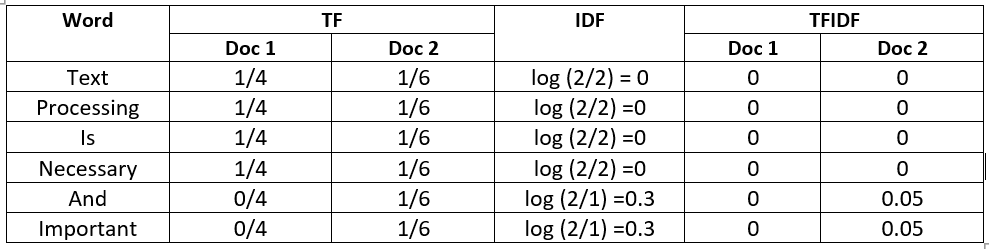
\includegraphics[scale=0.6]{../images/img_6.png} \\
        \href{https://www.analyticsvidhya.com/blog/2021/07/bag-of-words-vs-tfidf-vectorization-a-hands-on-tutorial/}{[Source of Example]}
    \end{center}

\end{frame}